% Following figures are from lxatut (CR-only background-only post-fit):
% /afs/cern.ch/work/z/zang/LQanalysis/taux_fastframes/run/script_codex/ch8_bonly_20260921/ch8_bonly/Plots/
% Source files: WCR_0tau1e0b_Res*_postFit.eps and WCR_0tau1e0b_Res*_postfit.yaml.
% Fit parameters and correlations were copied from:
% /afs/cern.ch/work/z/zang/LQanalysis/taux_fastframes/run/run_signal_scan/fit_results/TwoSided_HF0_3_HFSeperated_Renamed_unblind_BONLY/fit_taunub_sys_1l_allVR_BONLY_MU1500_gU1_5_23L0_2_alldecay_corrected_unblind/Fits/
% Local plot copies: data/ch8/bonly_20260921/Plots/; styling: scripts/ch8/restyle_bonly.py.
% Provenance and paper comparison: output/ch8/fit_audit_20260924/report.md.
\begin{figure}[htpb]
    \centering
    \begin{subfigure}{0.49\linewidth}
        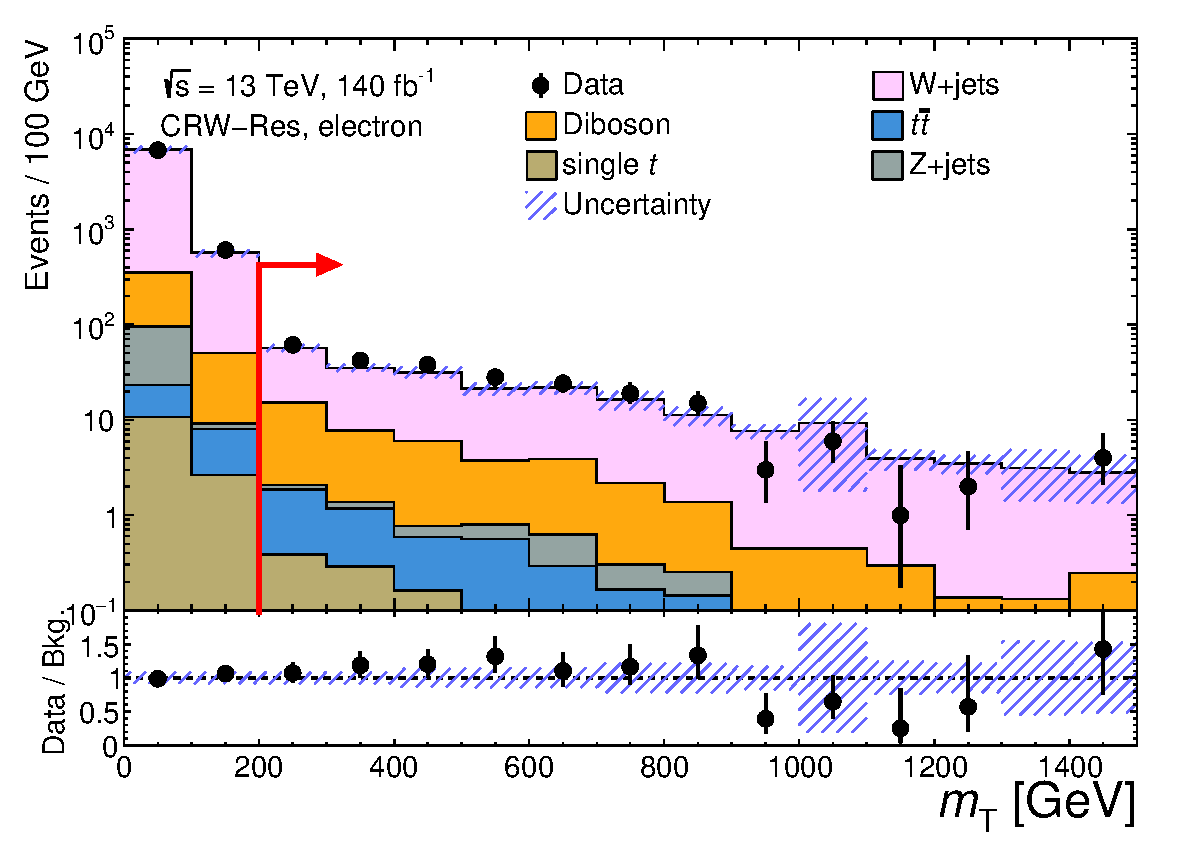
\includegraphics[width=\linewidth]{Figs/CH8/bonly/WCR_0tau1e0b_Res_mT_N_minus_1_mT.pdf}
        \caption[]{$\mT^\ell$.}
    \end{subfigure}\hfill
    \begin{subfigure}{0.49\linewidth}
        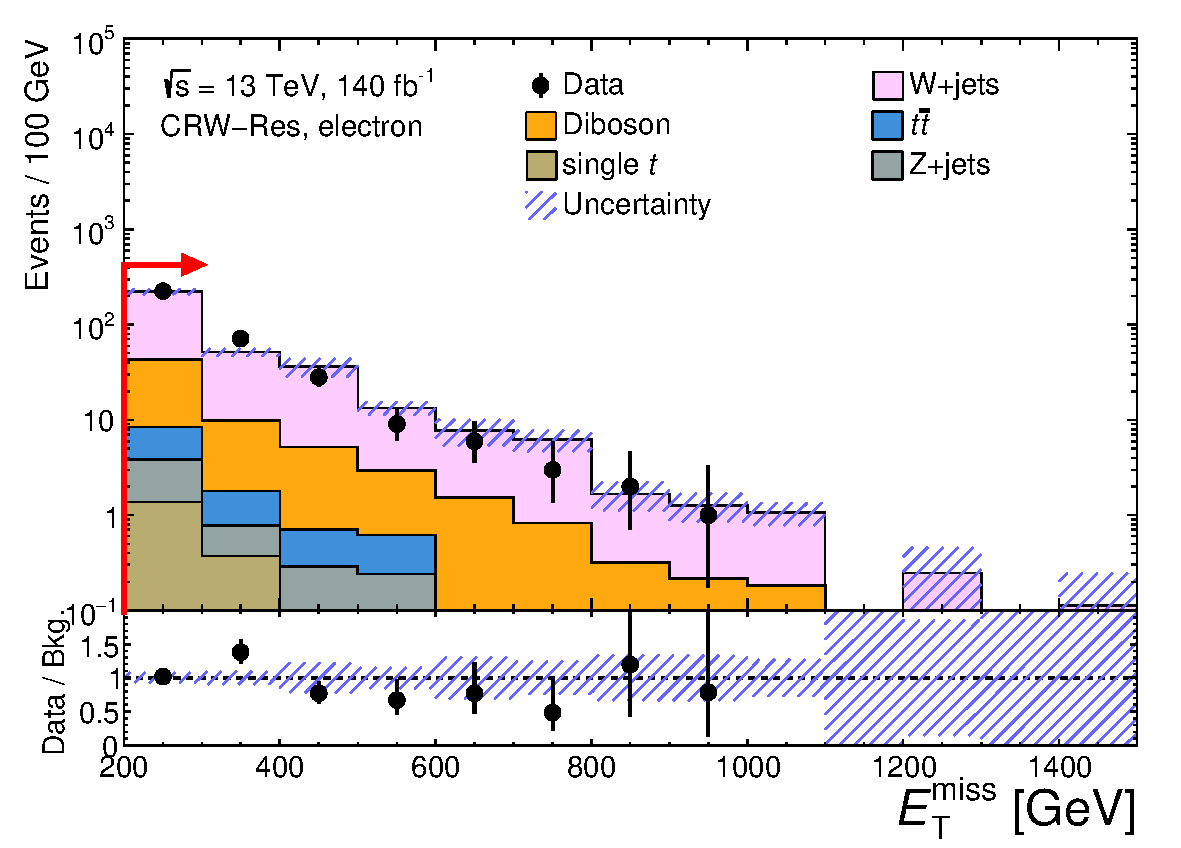
\includegraphics[width=\linewidth]{Figs/CH8/bonly/WCR_0tau1e0b_Res_met_N_minus_1_met.pdf}
        \caption[]{$\met$.}
    \end{subfigure}\\
    \begin{subfigure}{0.49\linewidth}
        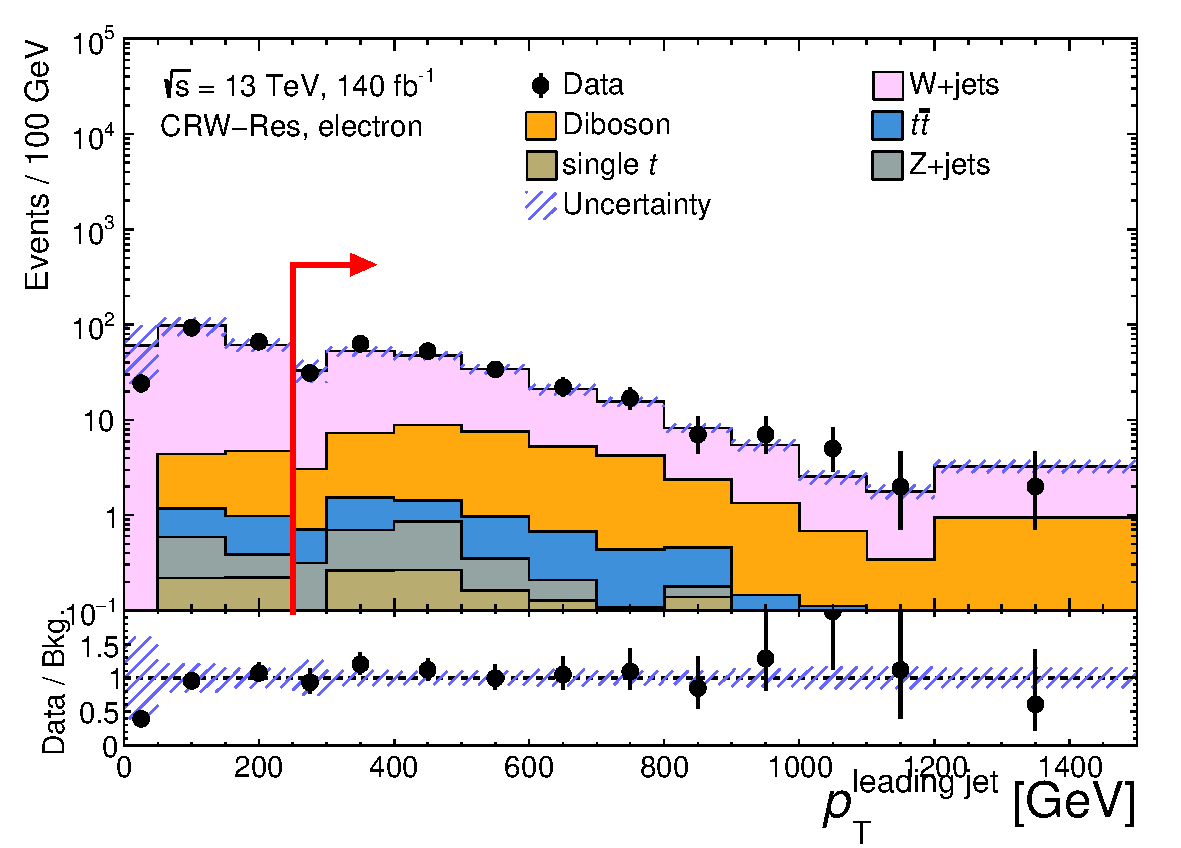
\includegraphics[width=\linewidth]{Figs/CH8/bonly/WCR_0tau1e0b_Res_jet_pT_0_N_minus_1_jet_pt_0.pdf}
        \caption[]{$\pT^{j_1}$.}
    \end{subfigure}\hfill
    \begin{subfigure}{0.49\linewidth}
        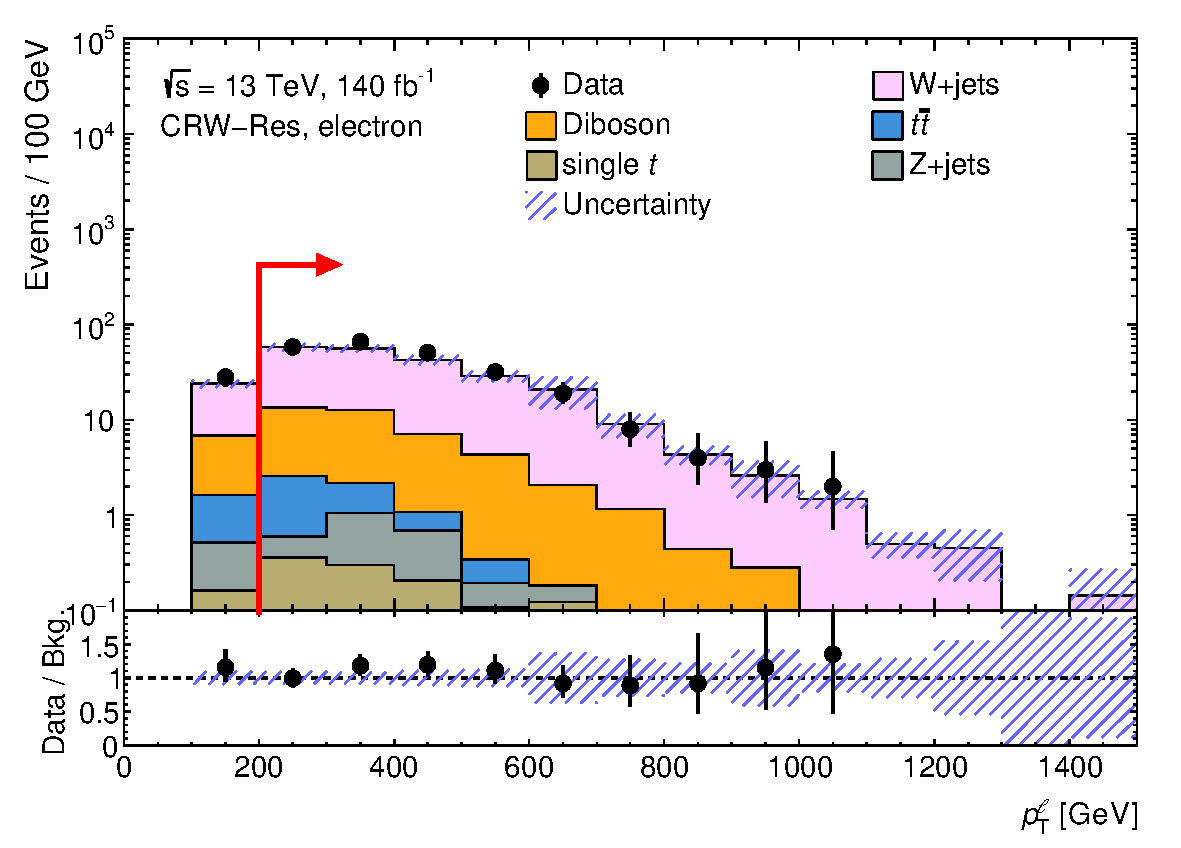
\includegraphics[width=\linewidth]{Figs/CH8/bonly/WCR_0tau1e0b_Res_lep_pT_N_minus_1_lep_pt_0.pdf}
        \caption[]{$\pT^\ell$.}
    \end{subfigure}\\
    \begin{subfigure}{0.49\linewidth}
        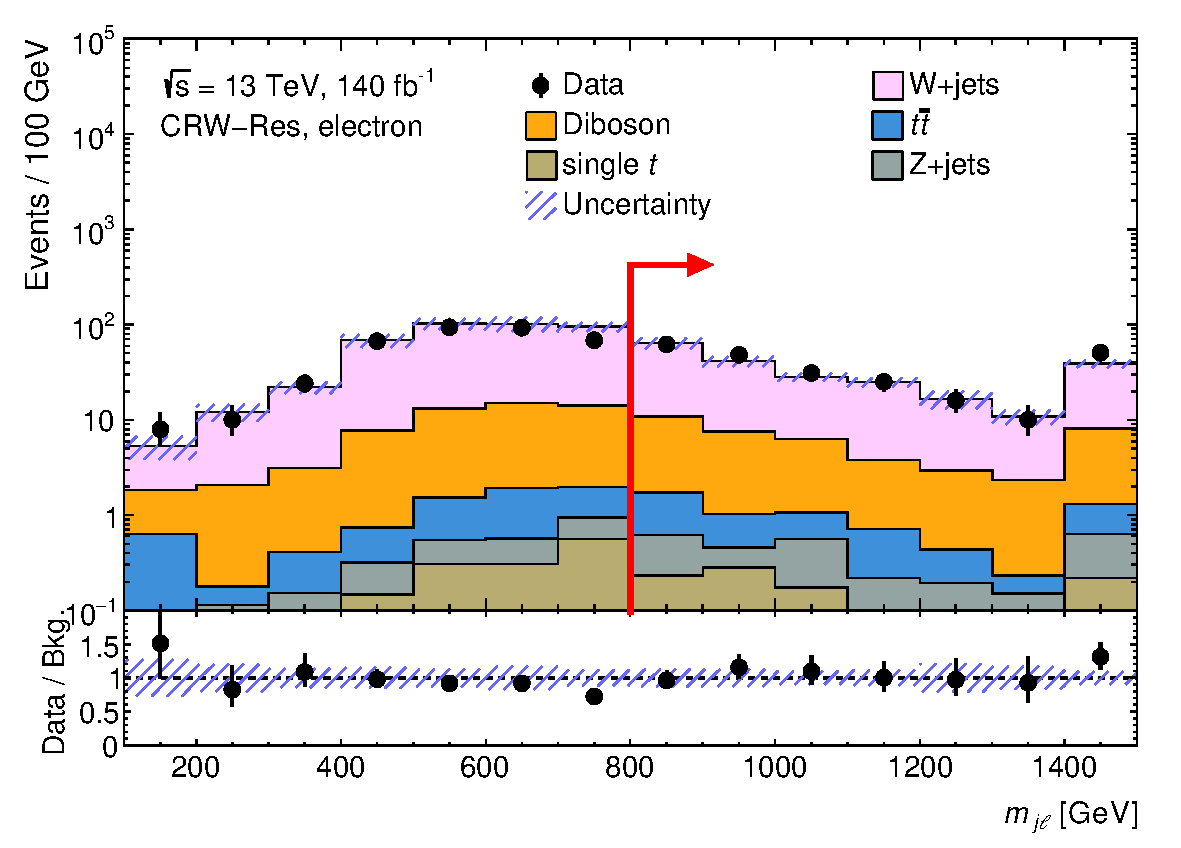
\includegraphics[width=\linewidth]{Figs/CH8/bonly/WCR_0tau1e0b_Res_InvM_N_minus_1_Mljet.pdf}
        \caption[]{$m_{j\ell}$.}
    \end{subfigure}\hfill
    \begin{subfigure}{0.49\linewidth}
        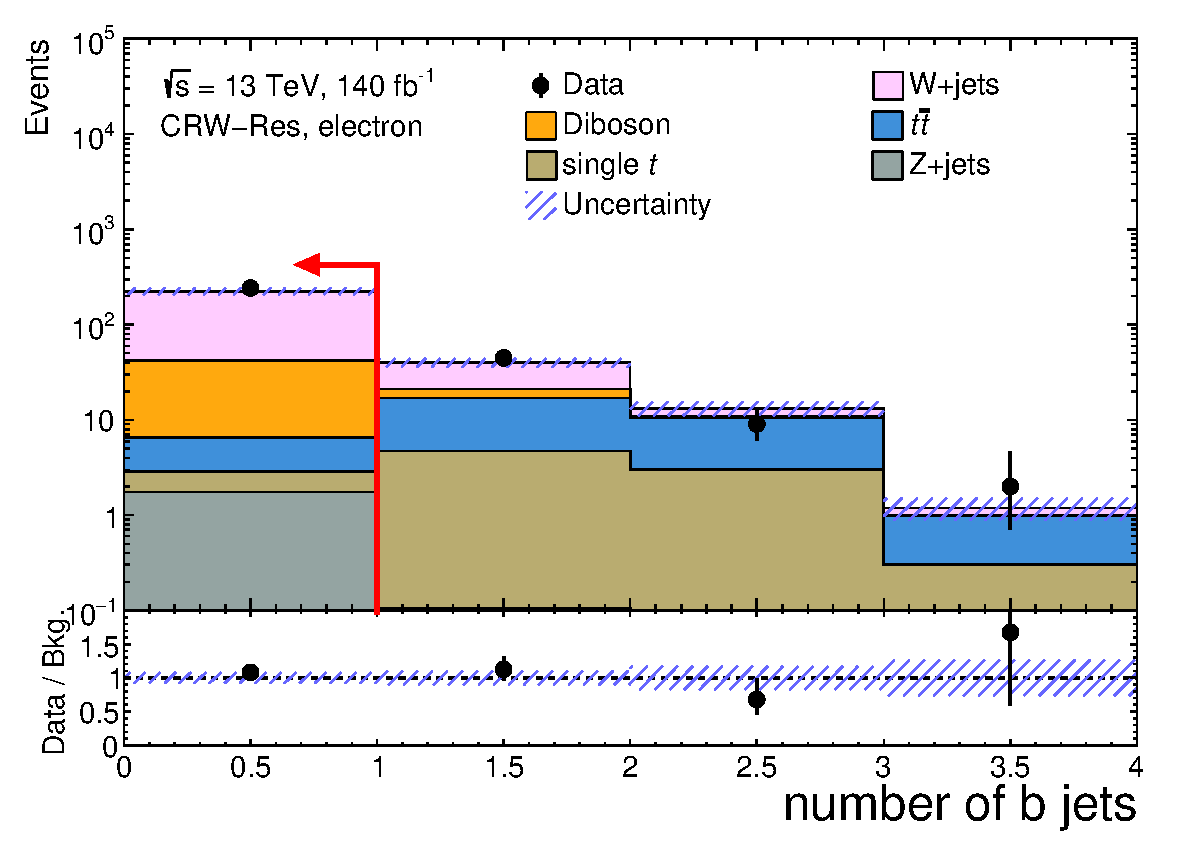
\includegraphics[width=\linewidth]{Figs/CH8/bonly/WCR_0tau1e0b_Res_n_bjets_N_minus_1_n_bjets.pdf}
        \caption[]{$N_b$.}
    \end{subfigure}
    \caption[Background-only fit distributions in CRW-Res, electron channel]{$N-1$ distributions in $\CRW$-$\Res$ for the $e$ channel, after the background-only fit in CRs. The hatched bands show the combined statistical and systematic uncertainties. The bottom panels show the ratio of data to background prediction. Red arrows indicate variable thresholds for the $\CRW$ regions. The last bin includes overflow.}
    \label{fig:ch8_wcr_res_e}
\end{figure}

% Following figures are from lxatut (CR-only background-only post-fit):
% /afs/cern.ch/work/z/zang/LQanalysis/taux_fastframes/run/script_codex/ch8_bonly_20260921/ch8_bonly/Plots/
% Source files: WCR_0tau1mu0b_Res*_postFit.eps and WCR_0tau1mu0b_Res*_postfit.yaml.
% Fit parameters and correlations were copied from:
% /afs/cern.ch/work/z/zang/LQanalysis/taux_fastframes/run/run_signal_scan/fit_results/TwoSided_HF0_3_HFSeperated_Renamed_unblind_BONLY/fit_taunub_sys_1l_allVR_BONLY_MU1500_gU1_5_23L0_2_alldecay_corrected_unblind/Fits/
% Local plot copies: data/ch8/bonly_20260921/Plots/; styling: scripts/ch8/restyle_bonly.py.
% Provenance and paper comparison: output/ch8/fit_audit_20260924/report.md.
\begin{figure}[htpb]
    \centering
    \begin{subfigure}{0.49\linewidth}
        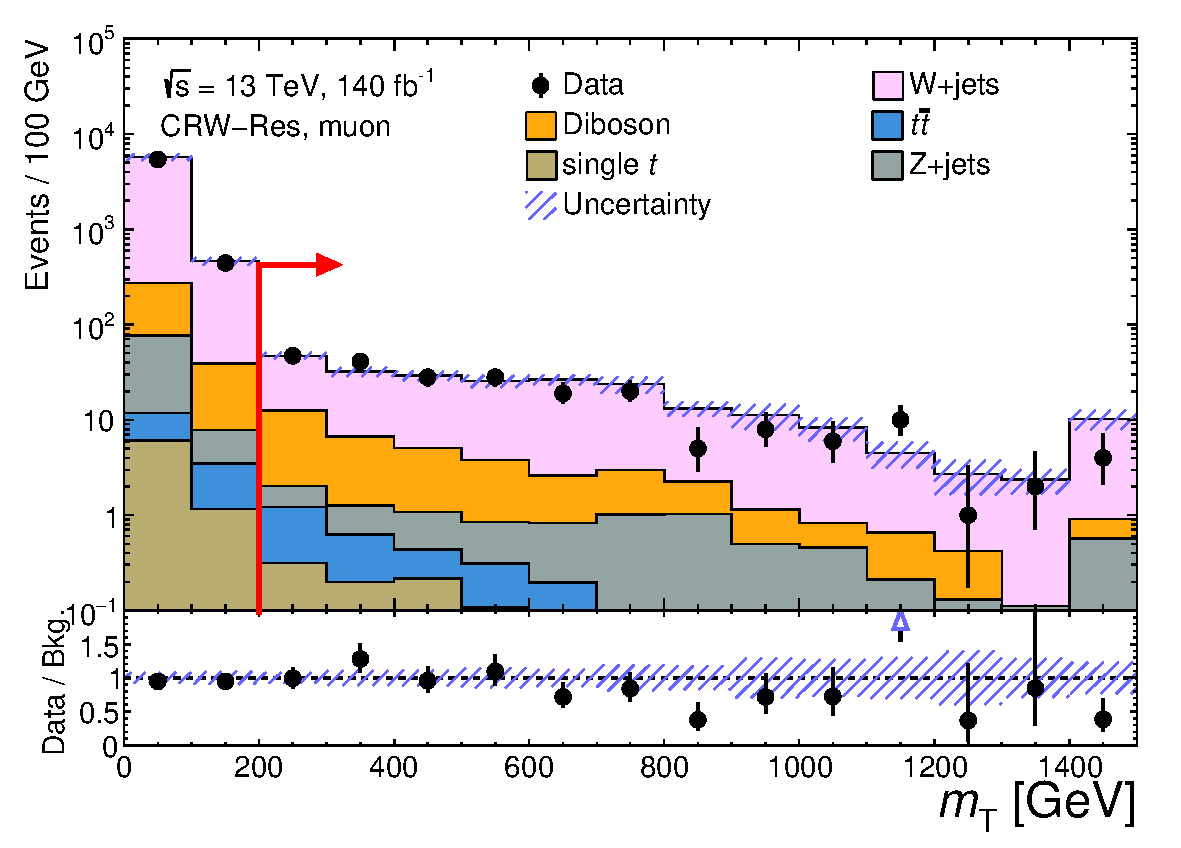
\includegraphics[width=\linewidth]{Figs/CH8/bonly/WCR_0tau1mu0b_Res_mT_N_minus_1_mT.pdf}
        \caption[]{$\mT^\ell$.}
    \end{subfigure}\hfill
    \begin{subfigure}{0.49\linewidth}
        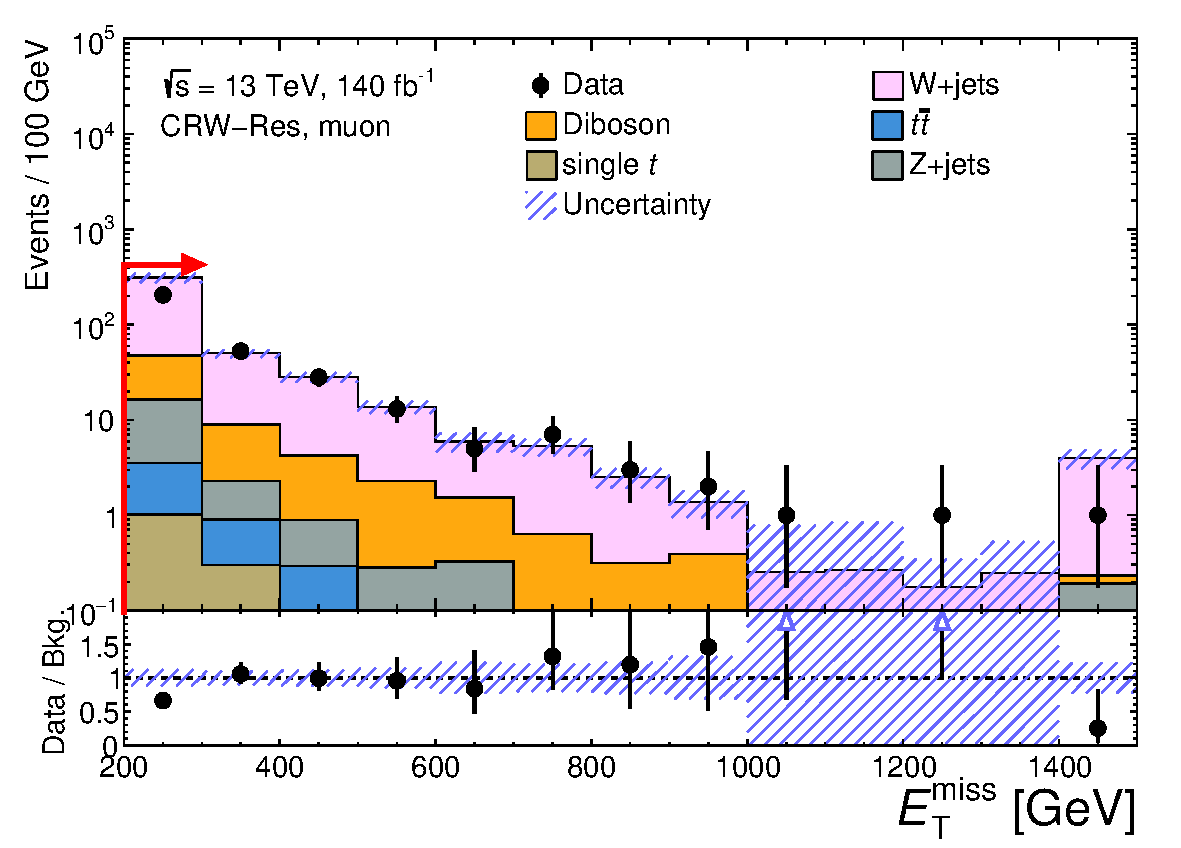
\includegraphics[width=\linewidth]{Figs/CH8/bonly/WCR_0tau1mu0b_Res_met_N_minus_1_met.pdf}
        \caption[]{$\met$.}
    \end{subfigure}\\
    \begin{subfigure}{0.49\linewidth}
        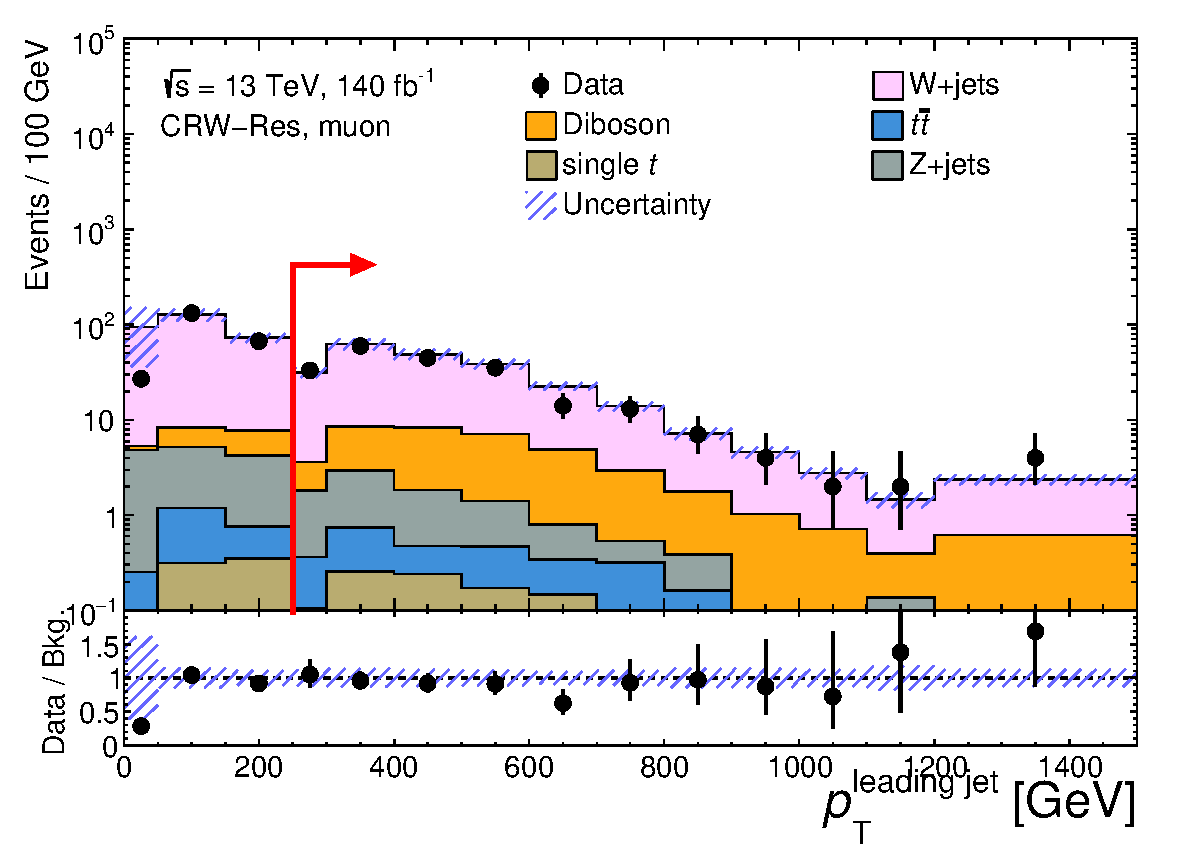
\includegraphics[width=\linewidth]{Figs/CH8/bonly/WCR_0tau1mu0b_Res_jet_pT_0_N_minus_1_jet_pt_0.pdf}
        \caption[]{$\pT^{j_1}$.}
    \end{subfigure}\hfill
    \begin{subfigure}{0.49\linewidth}
        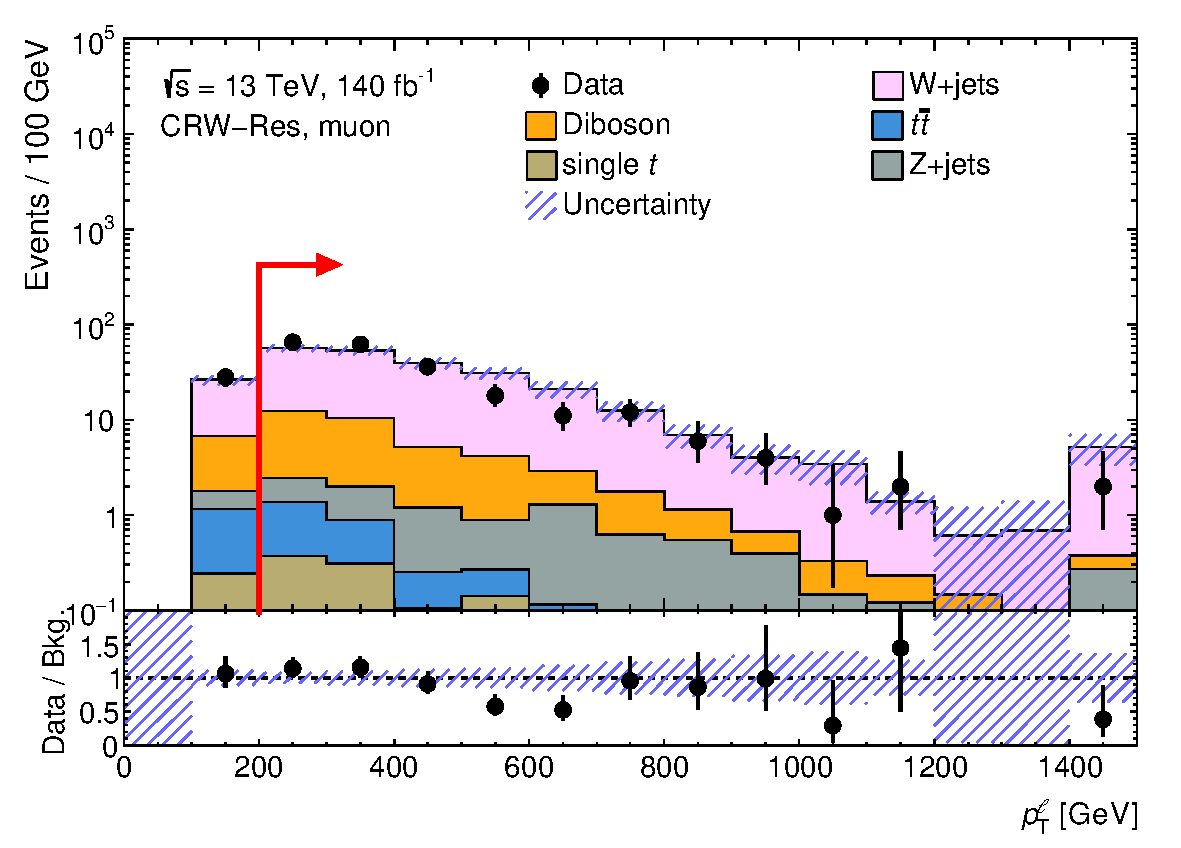
\includegraphics[width=\linewidth]{Figs/CH8/bonly/WCR_0tau1mu0b_Res_lep_pT_N_minus_1_lep_pt_0.pdf}
        \caption[]{$\pT^\ell$.}
    \end{subfigure}\\
    \begin{subfigure}{0.49\linewidth}
        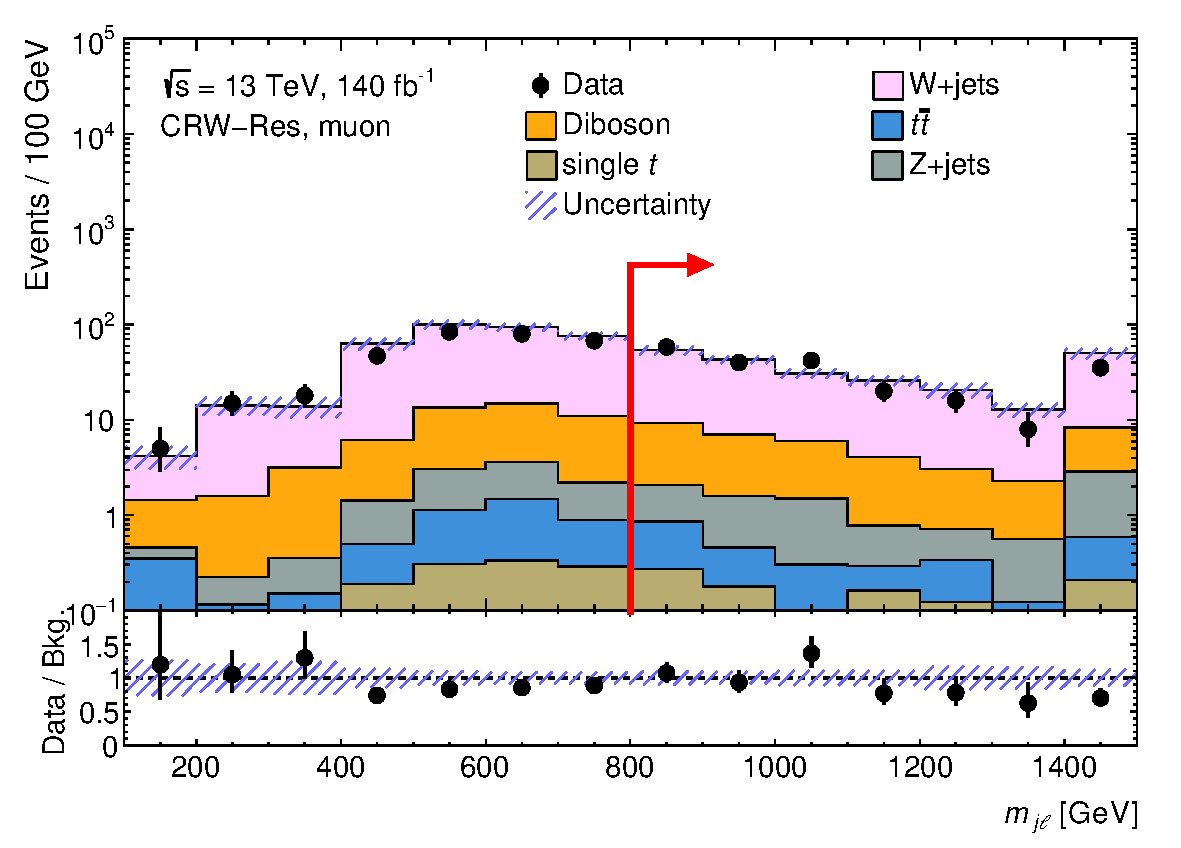
\includegraphics[width=\linewidth]{Figs/CH8/bonly/WCR_0tau1mu0b_Res_InvM_N_minus_1_Mljet.pdf}
        \caption[]{$m_{j\ell}$.}
    \end{subfigure}\hfill
    \begin{subfigure}{0.49\linewidth}
        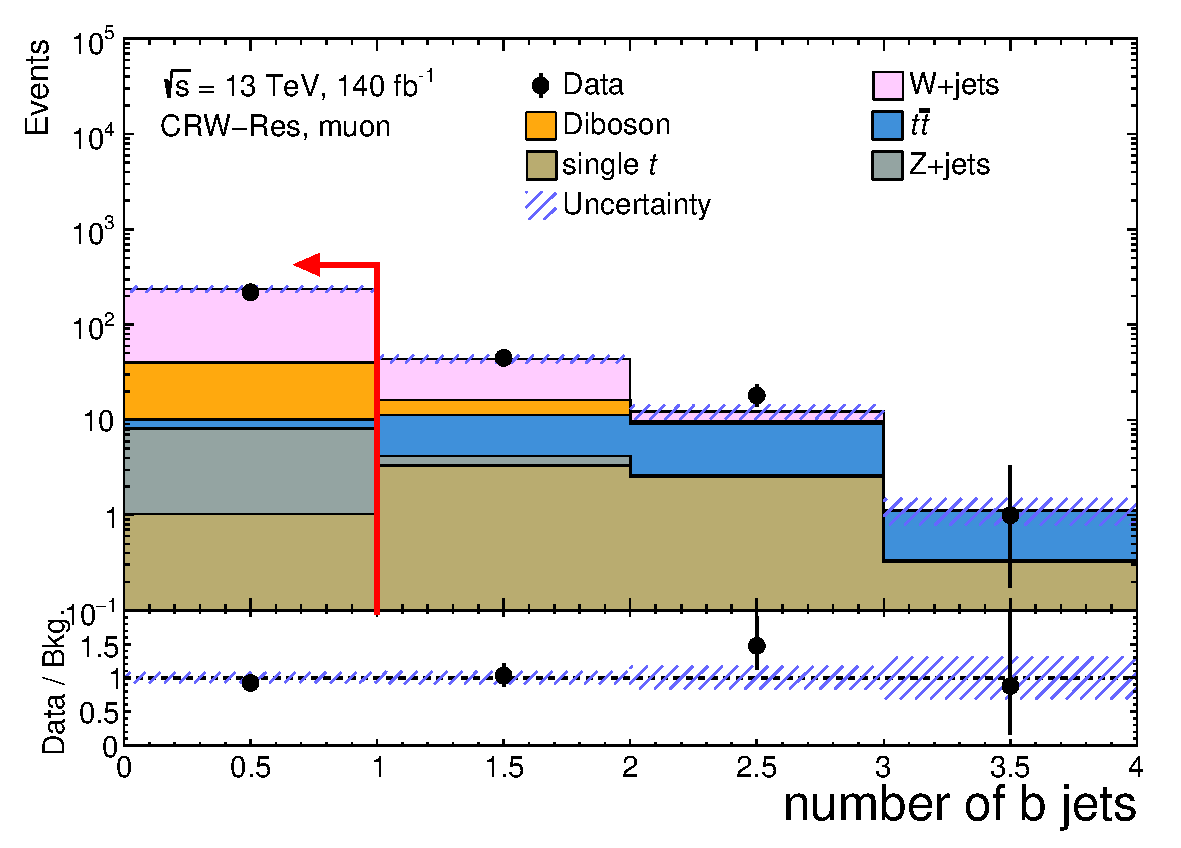
\includegraphics[width=\linewidth]{Figs/CH8/bonly/WCR_0tau1mu0b_Res_n_bjets_N_minus_1_n_bjets.pdf}
        \caption[]{$N_b$.}
    \end{subfigure}
    \caption[Background-only fit distributions in CRW-Res, muon channel]{$N-1$ distributions in $\CRW$-$\Res$ for the $\mu$ channel, after the background-only fit in CRs. The hatched bands show the combined statistical and systematic uncertainties. The bottom panels show the ratio of data to background prediction. Red arrows indicate variable thresholds for the $\CRW$ regions. The last bin includes overflow.}
    \label{fig:ch8_wcr_res_mu}
\end{figure}

% Following figures are from lxatut (CR-only background-only post-fit):
% /afs/cern.ch/work/z/zang/LQanalysis/taux_fastframes/run/script_codex/ch8_bonly_20260921/ch8_bonly/Plots/
% Source files: WCR_0tau1e0b_NonRes*_postFit.eps and WCR_0tau1e0b_NonRes*_postfit.yaml.
% Fit parameters and correlations were copied from:
% /afs/cern.ch/work/z/zang/LQanalysis/taux_fastframes/run/run_signal_scan/fit_results/TwoSided_HF0_3_HFSeperated_Renamed_unblind_BONLY/fit_taunub_sys_1l_allVR_BONLY_MU1500_gU1_5_23L0_2_alldecay_corrected_unblind/Fits/
% Local plot copies: data/ch8/bonly_20260921/Plots/; styling: scripts/ch8/restyle_bonly.py.
% Provenance and paper comparison: output/ch8/fit_audit_20260924/report.md.
\begin{figure}[htpb]
    \centering
    \begin{subfigure}{0.49\linewidth}
        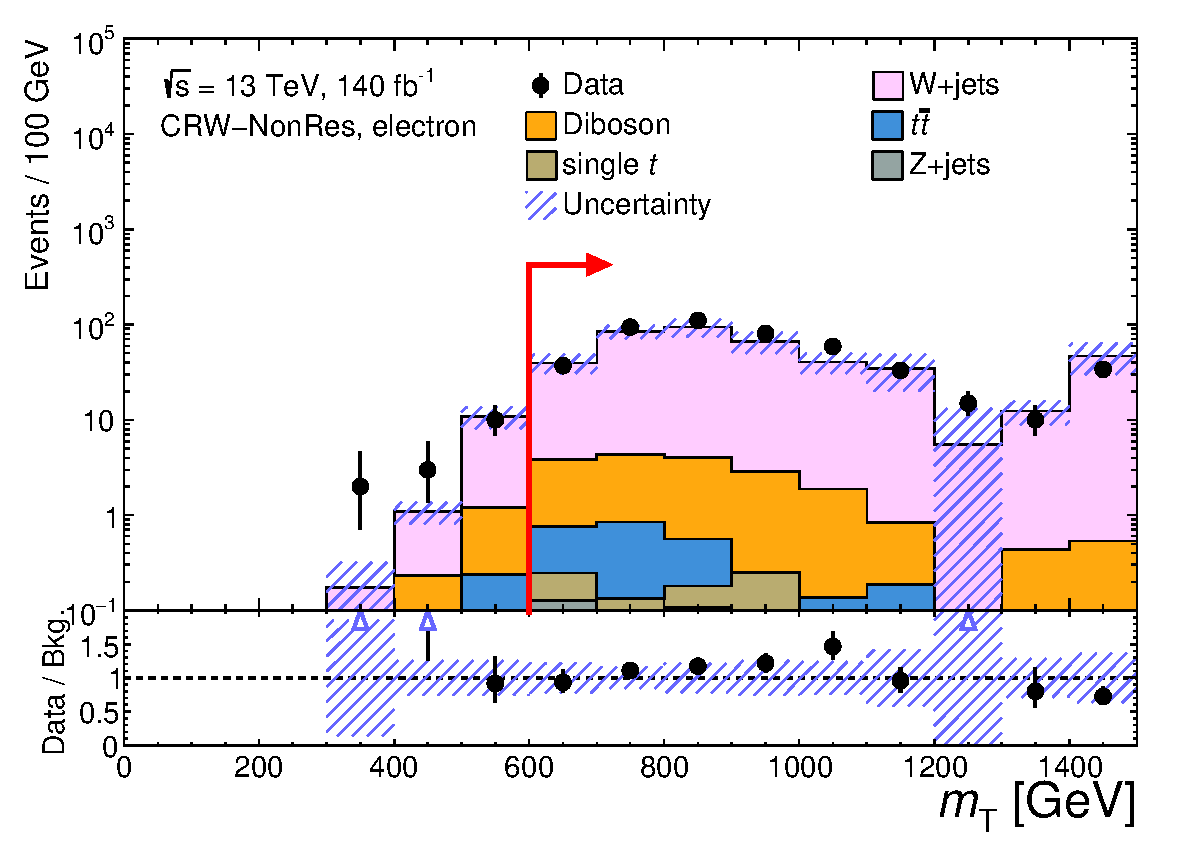
\includegraphics[width=\linewidth]{Figs/CH8/bonly/WCR_0tau1e0b_NonRes_mT_N_minus_1_mT.pdf}
        \caption[]{$\mT^\ell$.}
    \end{subfigure}\hfill
    \begin{subfigure}{0.49\linewidth}
        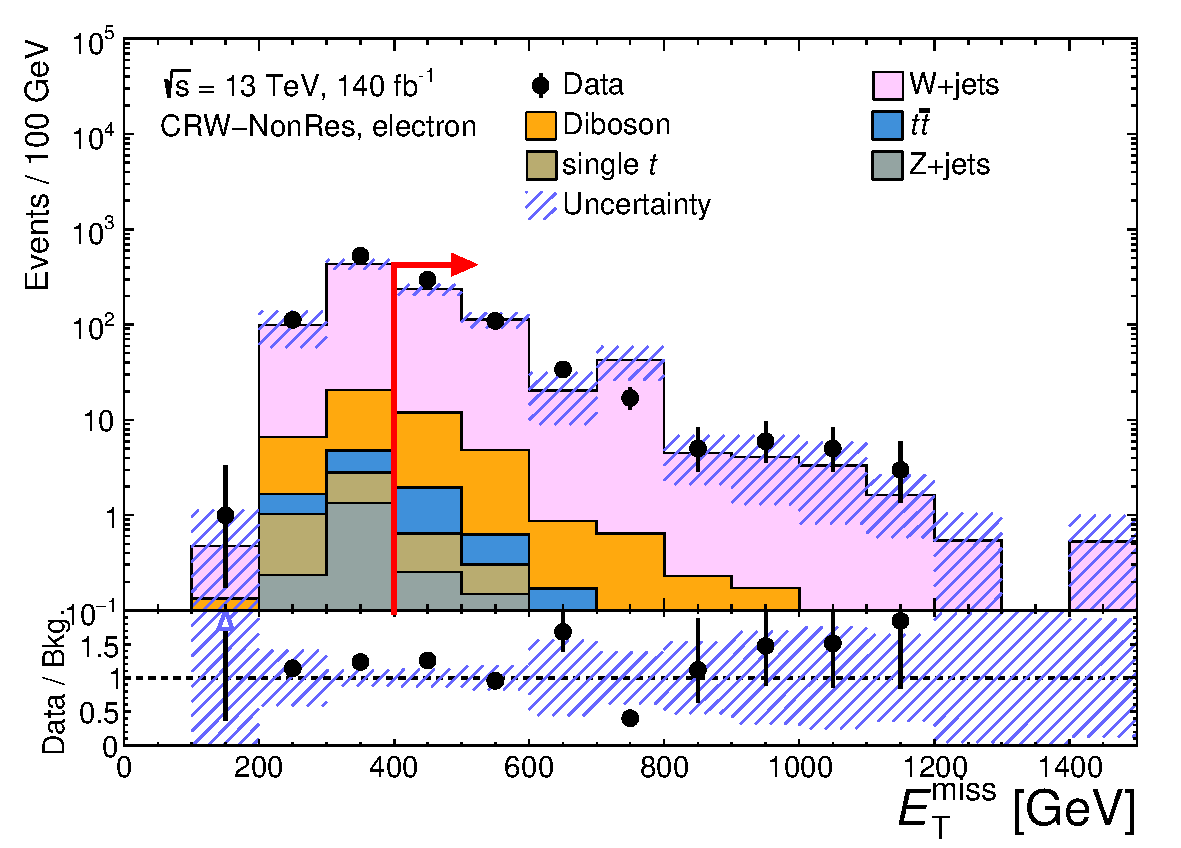
\includegraphics[width=\linewidth]{Figs/CH8/bonly/WCR_0tau1e0b_NonRes_met_N_minus_1_met.pdf}
        \caption[]{$\met$.}
    \end{subfigure}\\
    \begin{subfigure}{0.49\linewidth}
        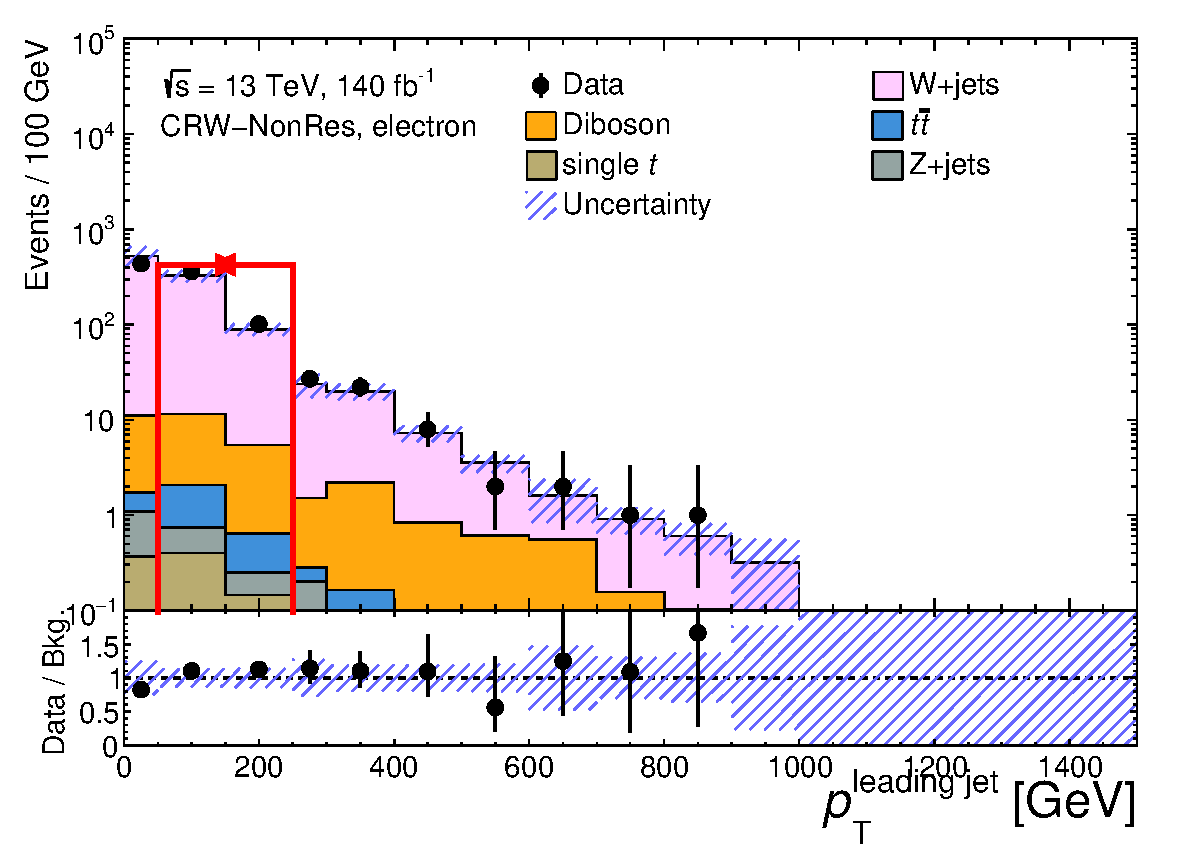
\includegraphics[width=\linewidth]{Figs/CH8/bonly/WCR_0tau1e0b_NonRes_jet_pT_0_N_minus_1_jet_pt_0.pdf}
        \caption[]{$\pT^{j_1}$.}
    \end{subfigure}\hfill
    \begin{subfigure}{0.49\linewidth}
        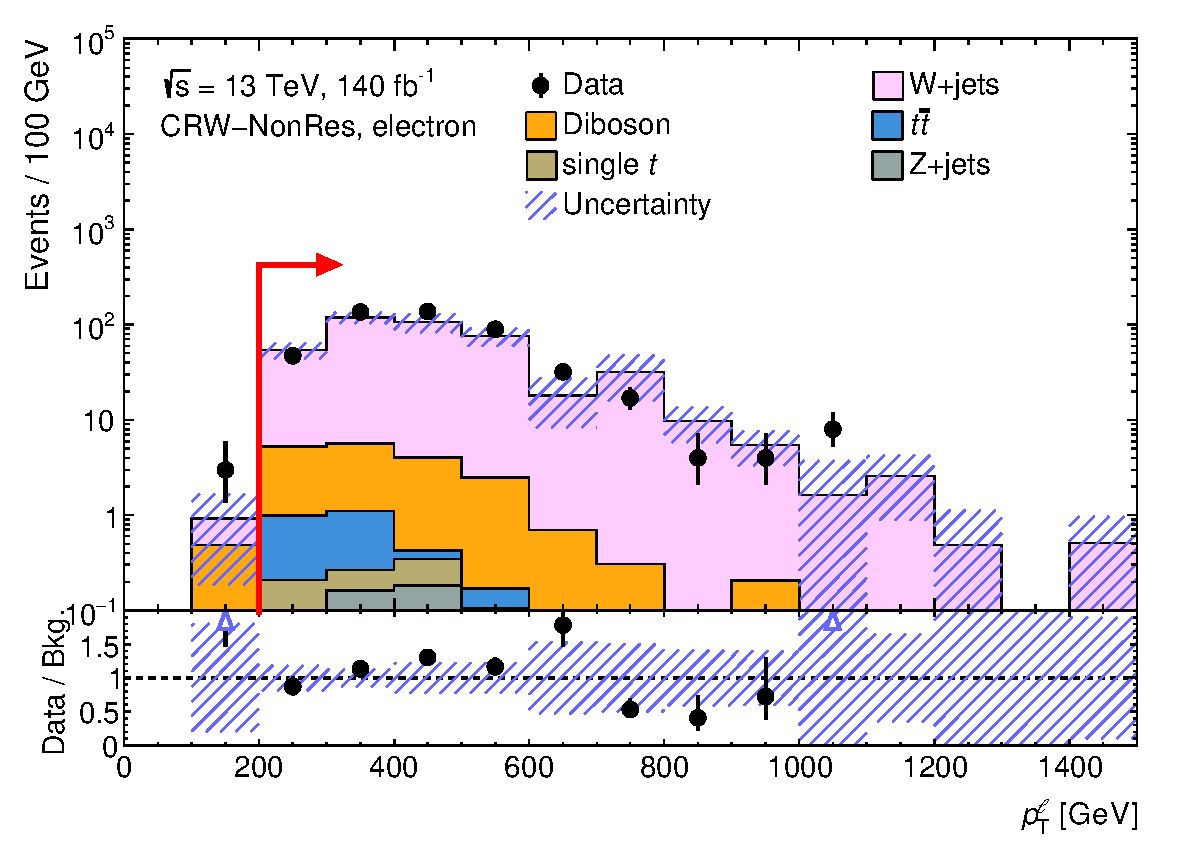
\includegraphics[width=\linewidth]{Figs/CH8/bonly/WCR_0tau1e0b_NonRes_lep_pT_N_minus_1_lep_pt_0.pdf}
        \caption[]{$\pT^\ell$.}
    \end{subfigure}\\
    \begin{subfigure}{0.49\linewidth}
        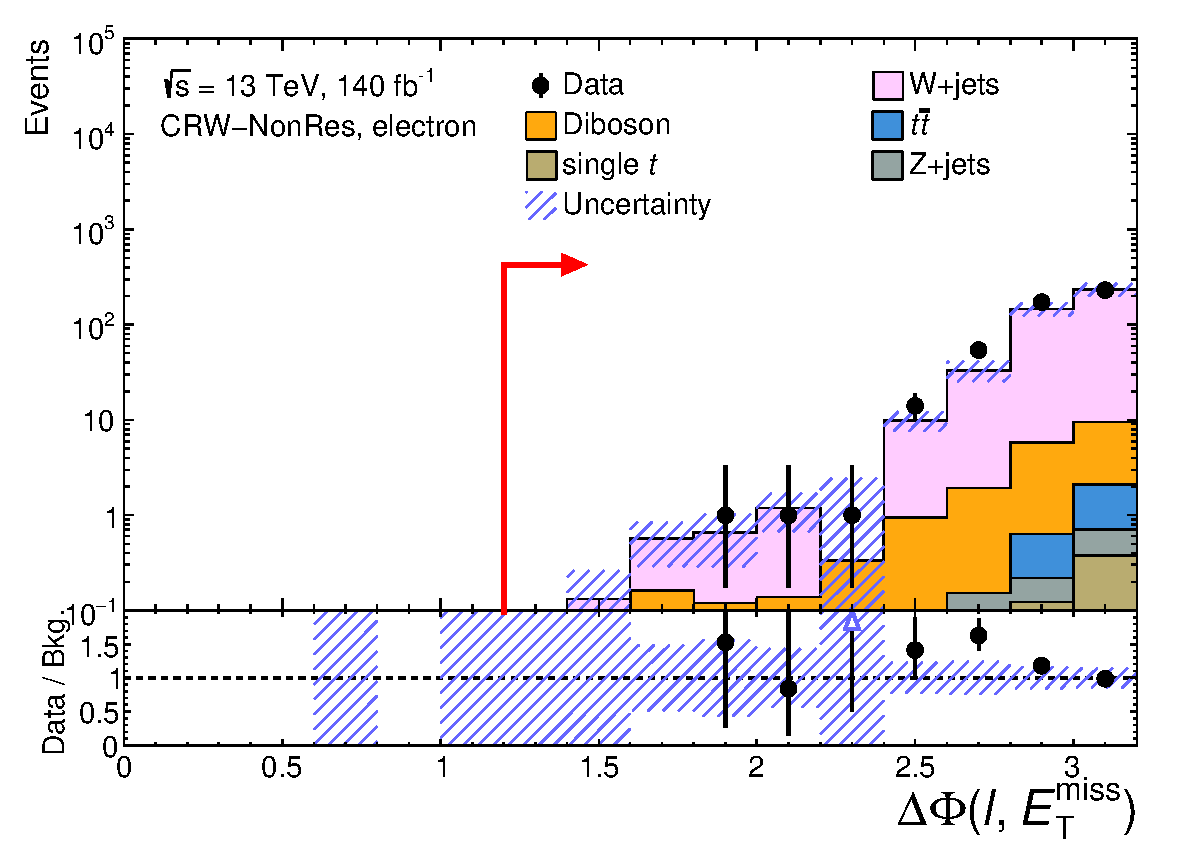
\includegraphics[width=\linewidth]{Figs/CH8/bonly/WCR_0tau1e0b_NonRes_DeltaPhi_N_minus_1_dphi_lmet.pdf}
        \caption[]{$\DphiLepMet$.}
    \end{subfigure}\hfill
    \begin{subfigure}{0.49\linewidth}
        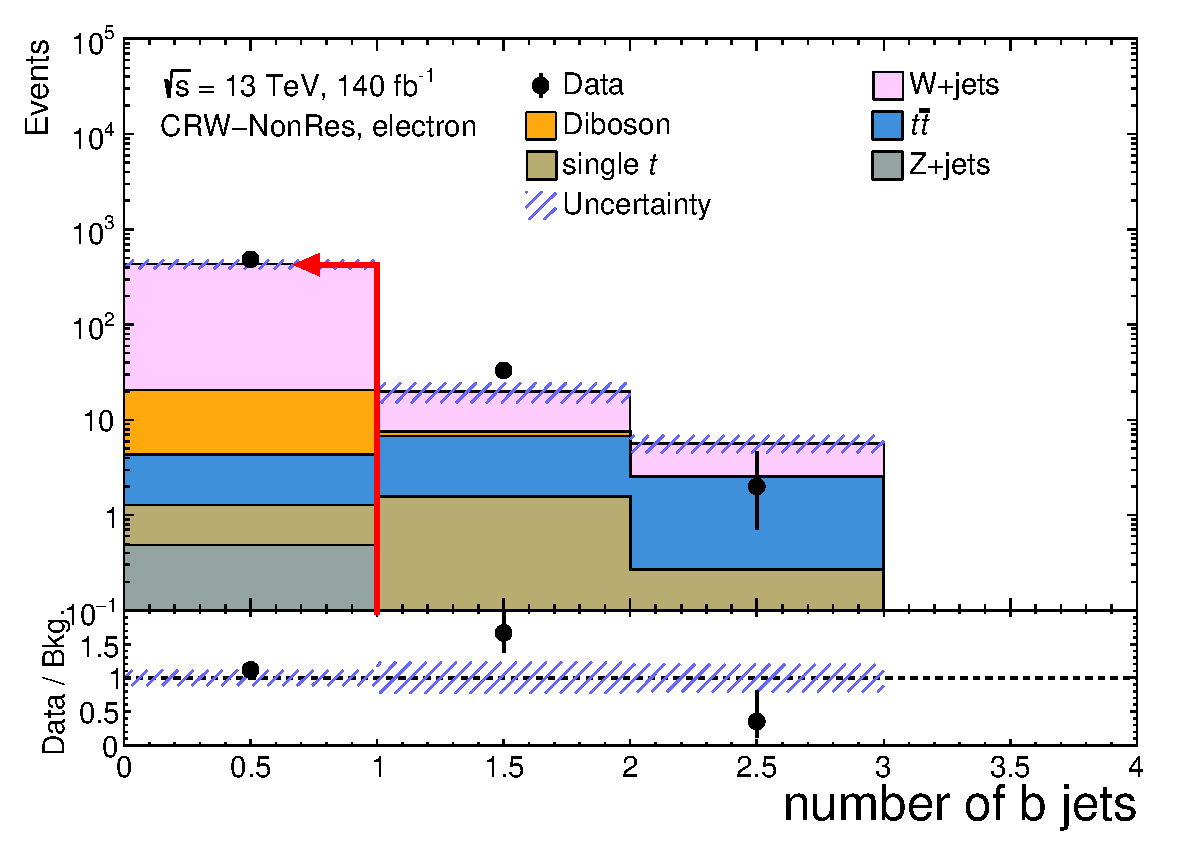
\includegraphics[width=\linewidth]{Figs/CH8/bonly/WCR_0tau1e0b_NonRes_n_bjets_N_minus_1_n_bjets.pdf}
        \caption[]{$N_b$.}
    \end{subfigure}
    \caption[Background-only fit distributions in CRW-NonRes, electron channel]{$N-1$ distributions in $\CRW$-$\NonRes$ for the $e$ channel, after the background-only fit in CRs. The hatched bands show the combined statistical and systematic uncertainties. The bottom panels show the ratio of data to background prediction. Red arrows indicate variable thresholds for the $\CRW$ regions. The last bin includes overflow.}
    \label{fig:ch8_wcr_nonres_e}
\end{figure}

% Following figures are from lxatut (CR-only background-only post-fit):
% /afs/cern.ch/work/z/zang/LQanalysis/taux_fastframes/run/script_codex/ch8_bonly_20260921/ch8_bonly/Plots/
% Source files: WCR_0tau1mu0b_NonRes*_postFit.eps and WCR_0tau1mu0b_NonRes*_postfit.yaml.
% Fit parameters and correlations were copied from:
% /afs/cern.ch/work/z/zang/LQanalysis/taux_fastframes/run/run_signal_scan/fit_results/TwoSided_HF0_3_HFSeperated_Renamed_unblind_BONLY/fit_taunub_sys_1l_allVR_BONLY_MU1500_gU1_5_23L0_2_alldecay_corrected_unblind/Fits/
% Local plot copies: data/ch8/bonly_20260921/Plots/; styling: scripts/ch8/restyle_bonly.py.
% Provenance and paper comparison: output/ch8/fit_audit_20260924/report.md.
\begin{figure}[htpb]
    \centering
    \begin{subfigure}{0.49\linewidth}
        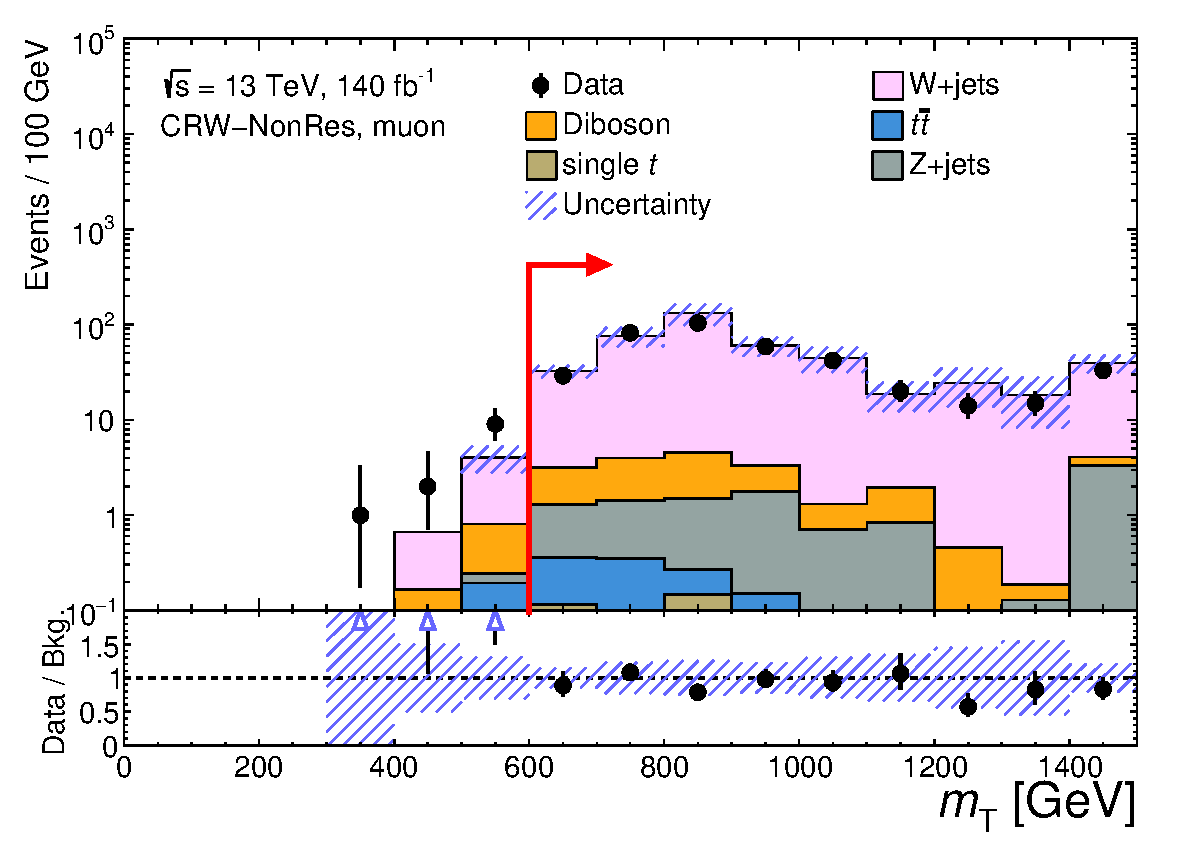
\includegraphics[width=\linewidth]{Figs/CH8/bonly/WCR_0tau1mu0b_NonRes_mT_N_minus_1_mT.pdf}
        \caption[]{$\mT^\ell$.}
    \end{subfigure}\hfill
    \begin{subfigure}{0.49\linewidth}
        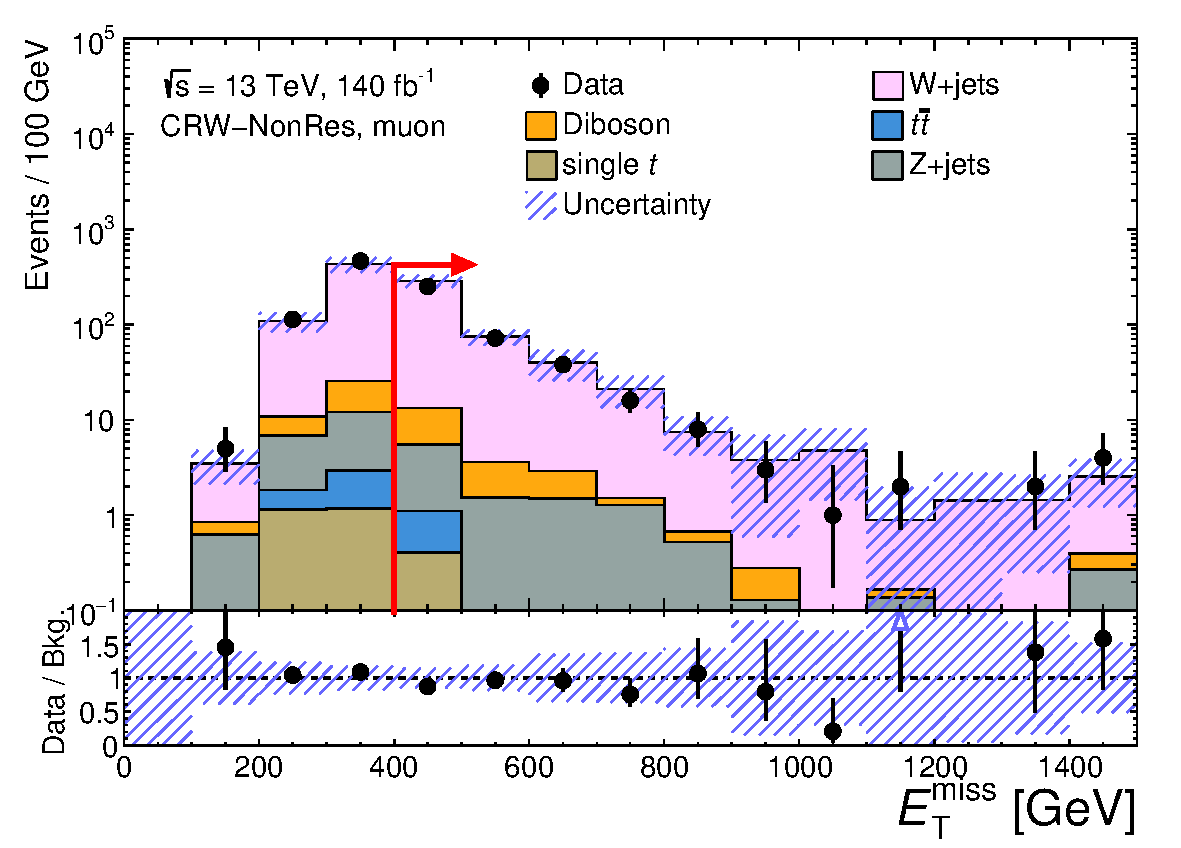
\includegraphics[width=\linewidth]{Figs/CH8/bonly/WCR_0tau1mu0b_NonRes_met_N_minus_1_met.pdf}
        \caption[]{$\met$.}
    \end{subfigure}\\
    \begin{subfigure}{0.49\linewidth}
        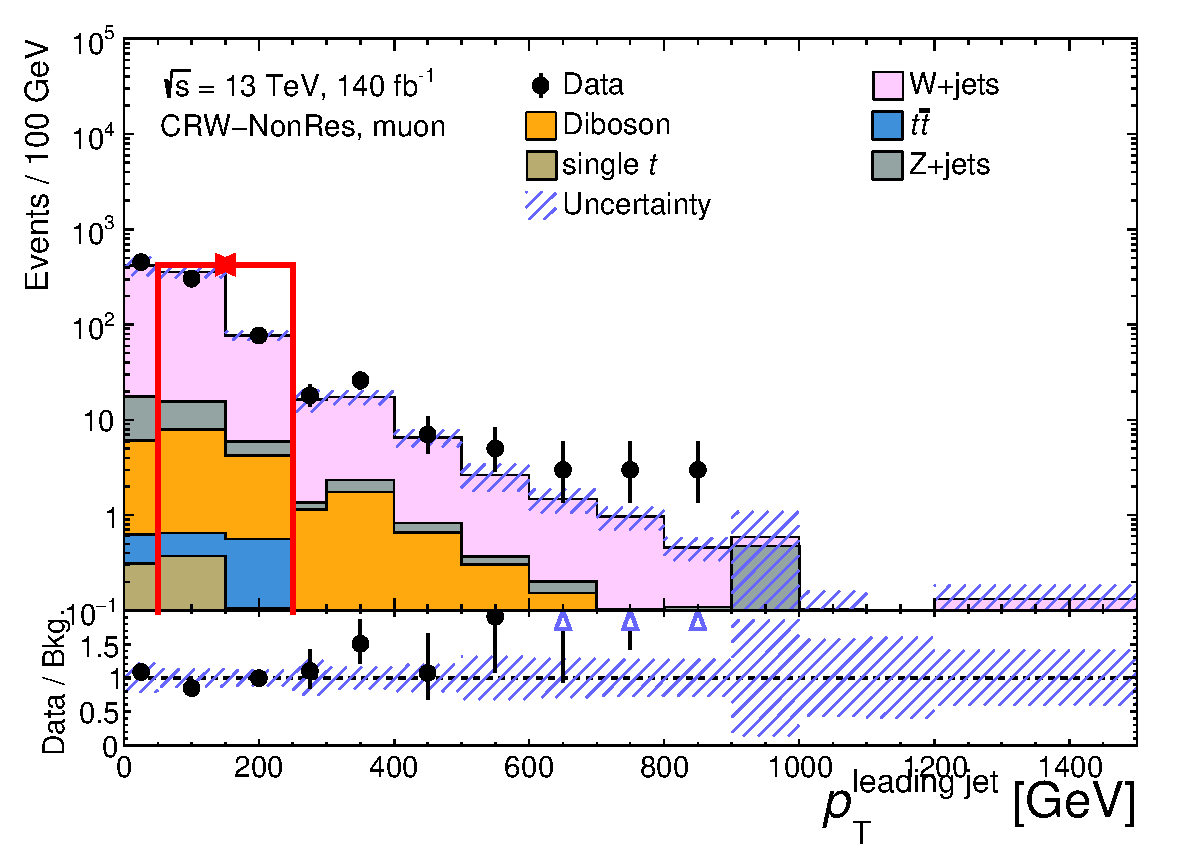
\includegraphics[width=\linewidth]{Figs/CH8/bonly/WCR_0tau1mu0b_NonRes_jet_pT_0_N_minus_1_jet_pt_0.pdf}
        \caption[]{$\pT^{j_1}$.}
        \label{fig:ch8_wcr_nonres_mu_jetpt}
    \end{subfigure}\hfill
    \begin{subfigure}{0.49\linewidth}
        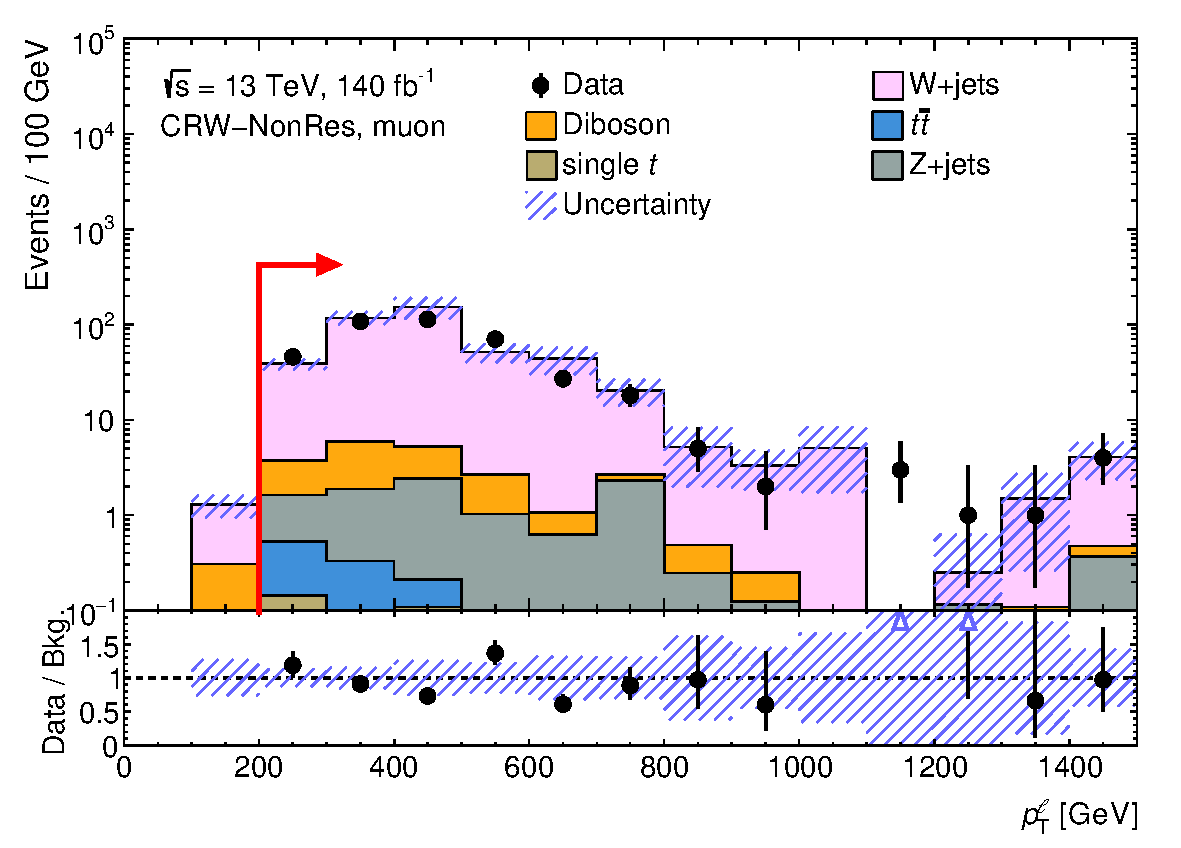
\includegraphics[width=\linewidth]{Figs/CH8/bonly/WCR_0tau1mu0b_NonRes_lep_pT_N_minus_1_lep_pt_0.pdf}
        \caption[]{$\pT^\ell$.}
    \end{subfigure}\\
    \begin{subfigure}{0.49\linewidth}
        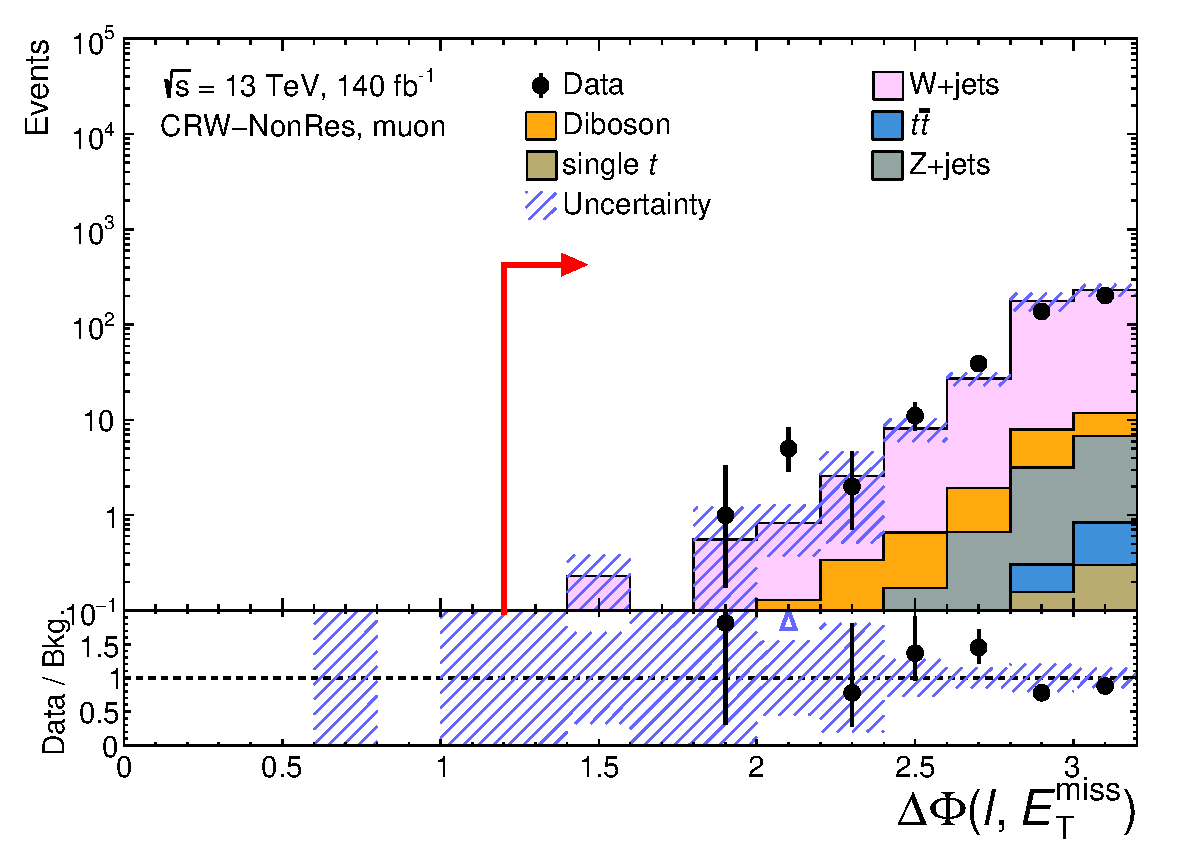
\includegraphics[width=\linewidth]{Figs/CH8/bonly/WCR_0tau1mu0b_NonRes_DeltaPhi_N_minus_1_dphi_lmet.pdf}
        \caption[]{$\DphiLepMet$.}
    \end{subfigure}\hfill
    \begin{subfigure}{0.49\linewidth}
        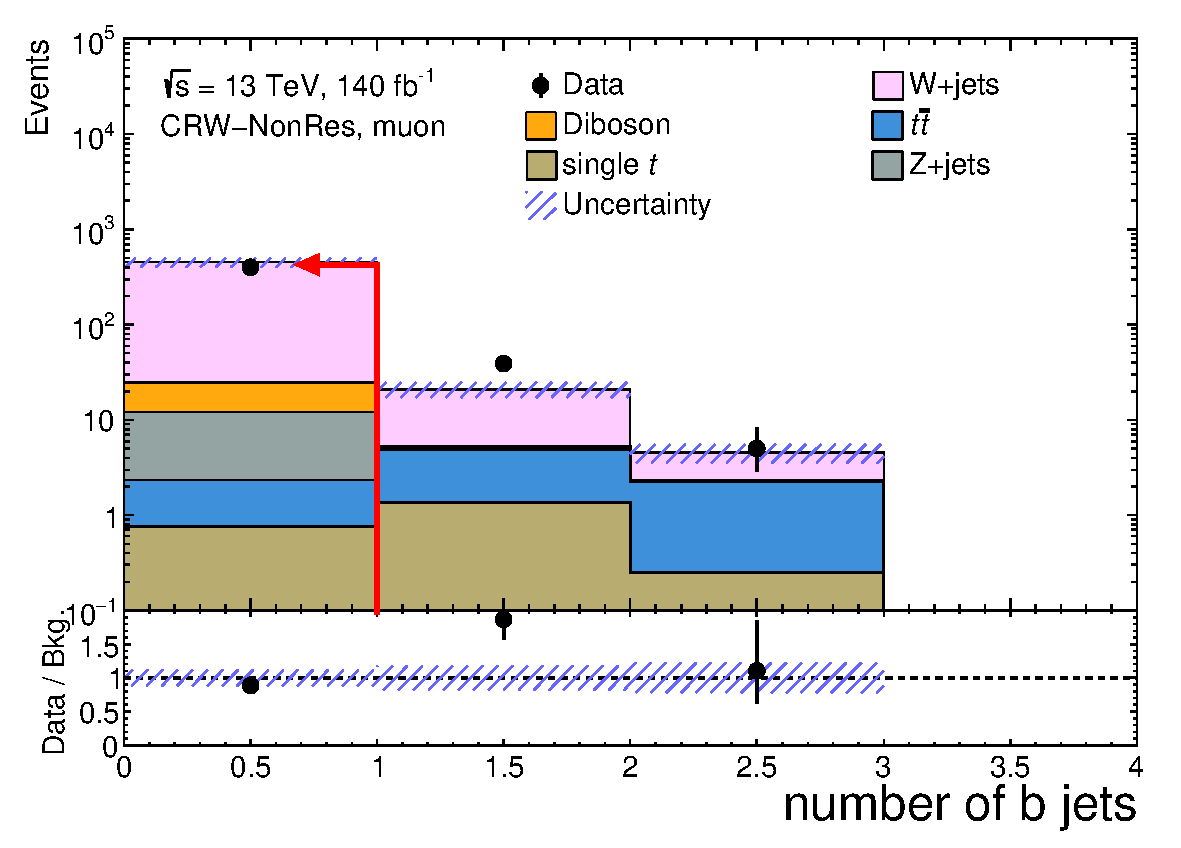
\includegraphics[width=\linewidth]{Figs/CH8/bonly/WCR_0tau1mu0b_NonRes_n_bjets_N_minus_1_n_bjets.pdf}
        \caption[]{$N_b$.}
    \end{subfigure}
    \caption[Background-only fit distributions in CRW-NonRes, muon channel]{$N-1$ distributions in $\CRW$-$\NonRes$ for the $\mu$ channel, after the background-only fit in CRs. The hatched bands show the combined statistical and systematic uncertainties. The bottom panels show the ratio of data to background prediction. Red arrows indicate variable thresholds for the $\CRW$ regions. The last bin includes overflow.}
    \label{fig:ch8_wcr_nonres_mu}
\end{figure}
